\documentclass[11pt,fleqn]{exam}

\setlength {\topmargin} {-.15in}
\setlength {\textheight} {8.6in}
\usepackage{enumerate}
\usepackage{amsmath}
\usepackage{amssymb}
\usepackage{xcolor}
\usepackage[colorlinks = true,
            linkcolor = blue,
            urlcolor  = blue,
            citecolor = blue,
            anchorcolor = blue]{hyperref}
\usepackage{listings}
\usepackage{color} %red, green, blue, yellow, cyan, magenta, black, white
\usepackage{graphicx}
\definecolor{mygreen}{RGB}{28,172,0} % color values Red, Green, Blue
\definecolor{mylilas}{RGB}{170,55,241}
\newcommand{\nn}{~\newline \noindent }
\newcommand{\mname}[1]{\mbox{\sf #1}}
\usepackage{float}


\begin{document}

\lstset{language=Matlab,%
    %basicstyle=\color{red},
    breaklines=true,%
    morekeywords={matlab2tikz},
    keywordstyle=\color{blue},%
    morekeywords=[2]{1}, keywordstyle=[2]{\color{black}},
    identifierstyle=\color{black},%
    stringstyle=\color{mylilas},
    commentstyle=\color{mygreen},%
    showstringspaces=false,%without this there will be a symbol in the places where there is a space
    numbers=none,%
    numberstyle={\tiny \color{black}},% size of the numbers
    numbersep=9pt, % this defines how far the numbers are from the text
    emph=[1]{for,end,break},emphstyle=[1]\color{red}, %some words to emphasise
    %emph=[2]{word1,word2}, emphstyle=[2]{style},    
}
	
\begin{center}
	{\large \textbf{COMPSCI 4X03}}\\[2mm]
	{\huge \textbf{Assignment 4}}\\[6mm]
	{\large \textbf{Mingzhe Wang}}\\[2mm]
	{\large \textbf{McMaster University}}\\[6mm]
	{\large \today}
		
\end{center}
	
	
% useful codes

%\begin{figure}[H]
%  	\centering
%  	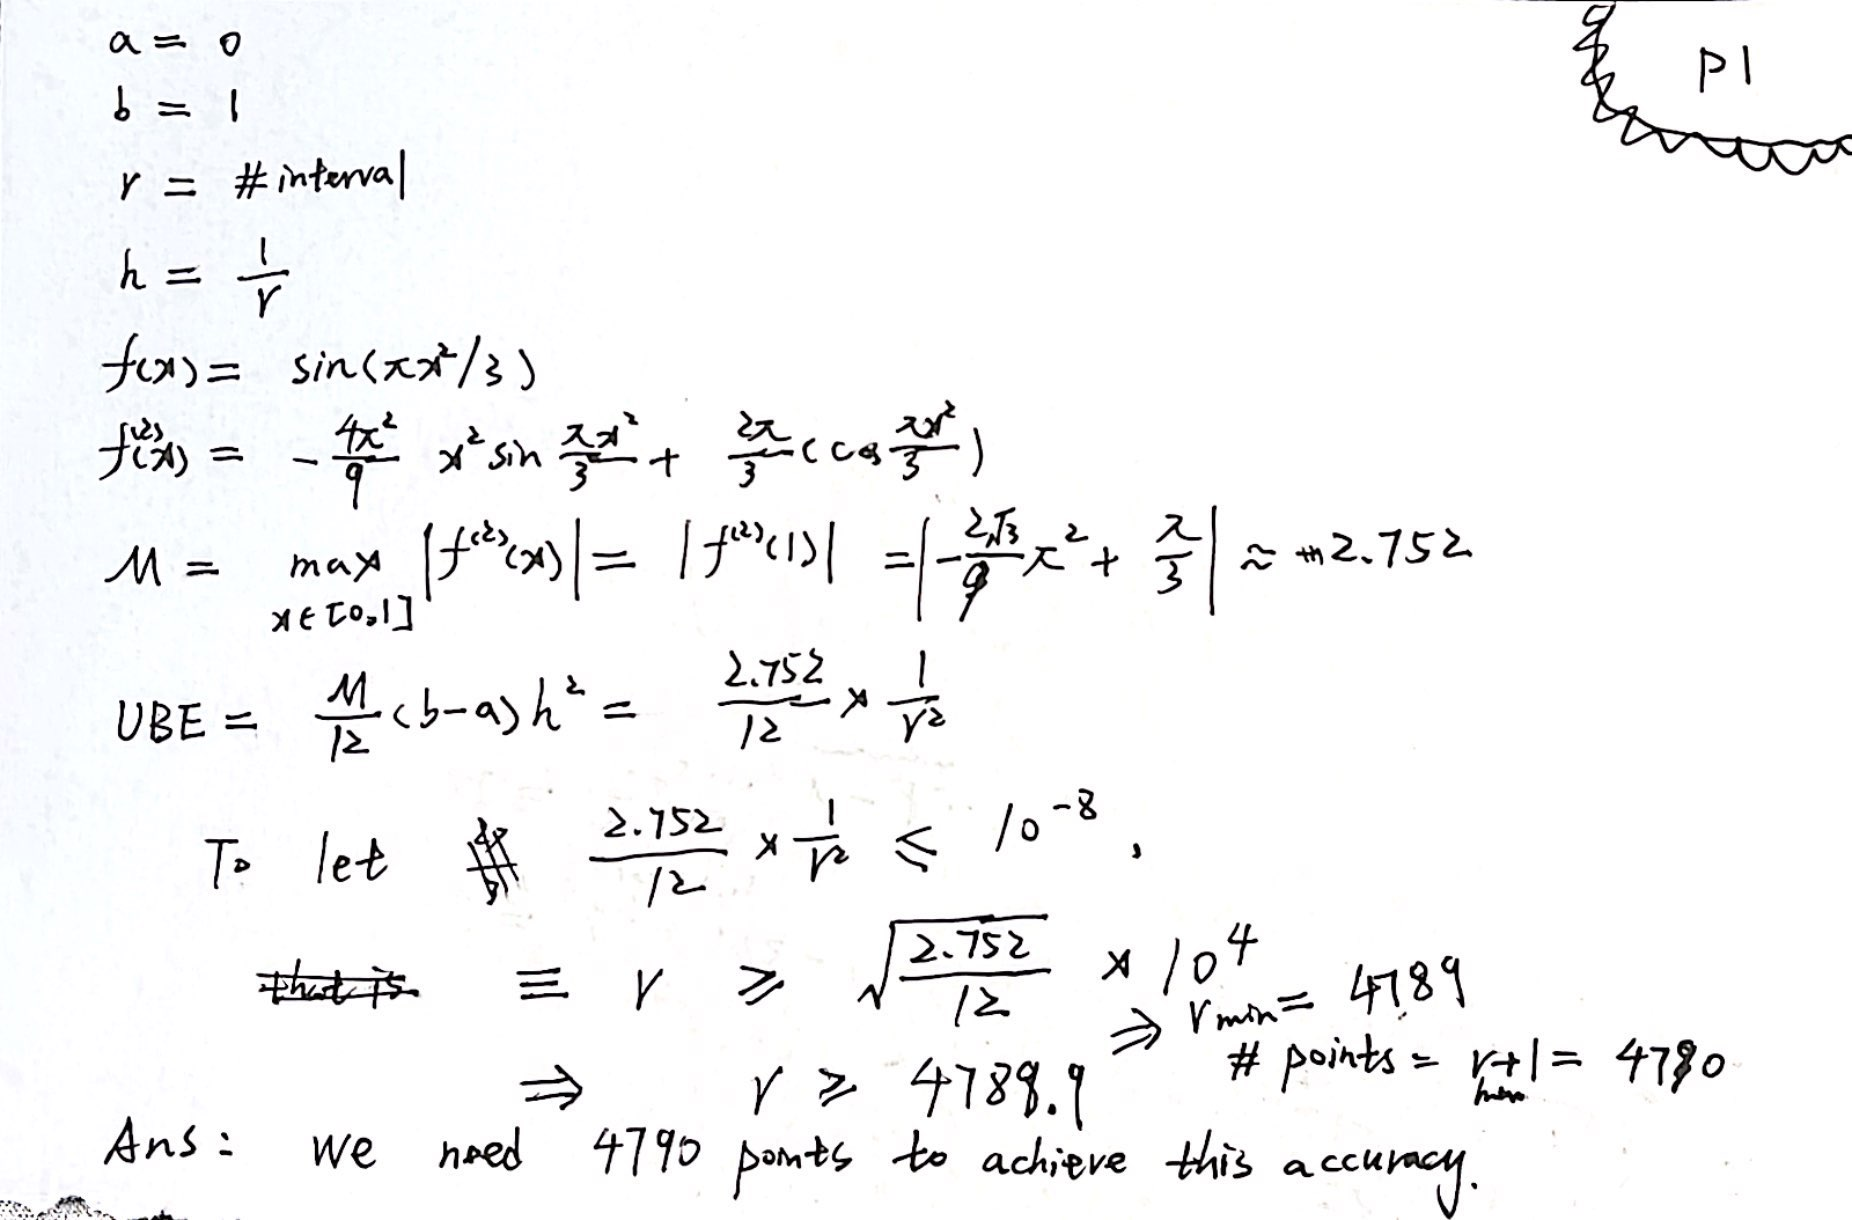
\includegraphics[width=1\textwidth]{p1.jpg}
%\end{figure}	

%\begin{lstlisting}
%midpoint 3.48e-02*h^2.00
%trapezoid 6.95e-02*h^2.00
%simpson 7.87e-03*h^3.97
%\end{lstlisting}

%\lstinputlisting{q3.m}
	
	
\medskip
		
\subsection*{Problem 1}
\subsubsection*{netbp2}
\lstinputlisting{netbp2.m}

\subsubsection*{classifypoints}
\lstinputlisting{classifypoints.m}

\subsubsection*{two plots}
\begin{figure}[H]
  	\centering
  	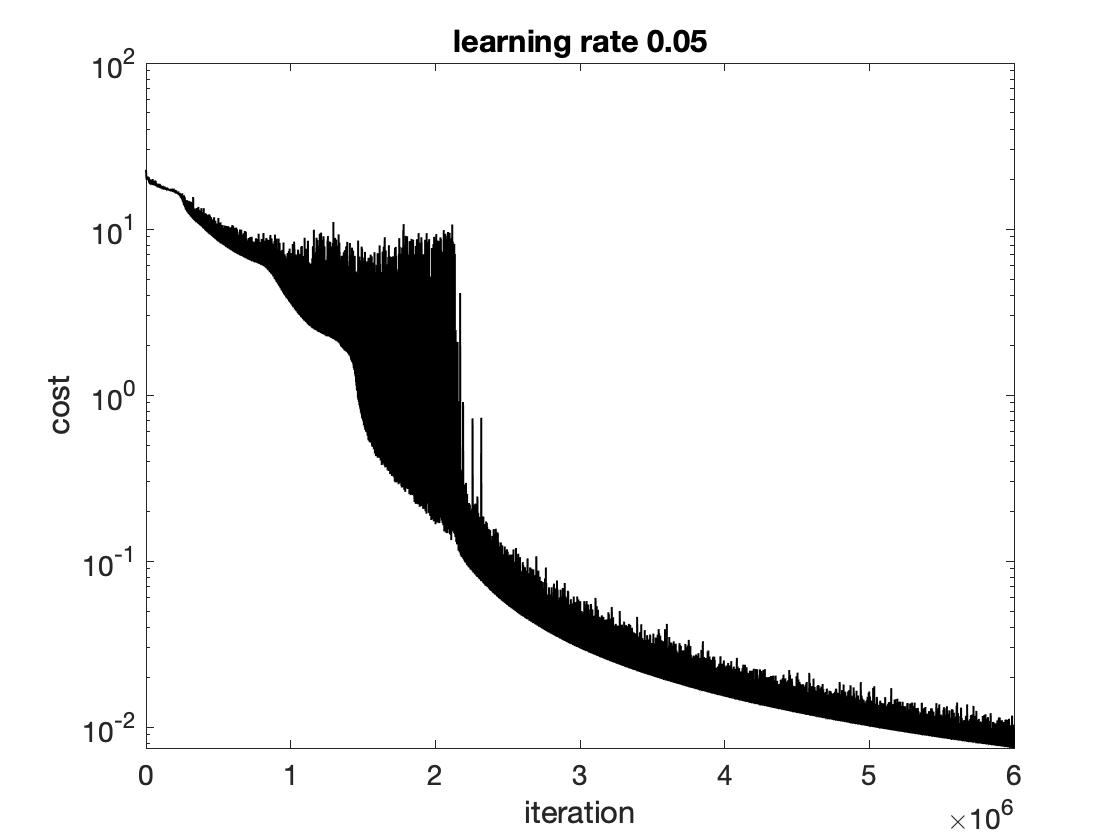
\includegraphics[width=1\textwidth]{q11.jpg}
\end{figure}	

\begin{figure}[H]
  	\centering
  	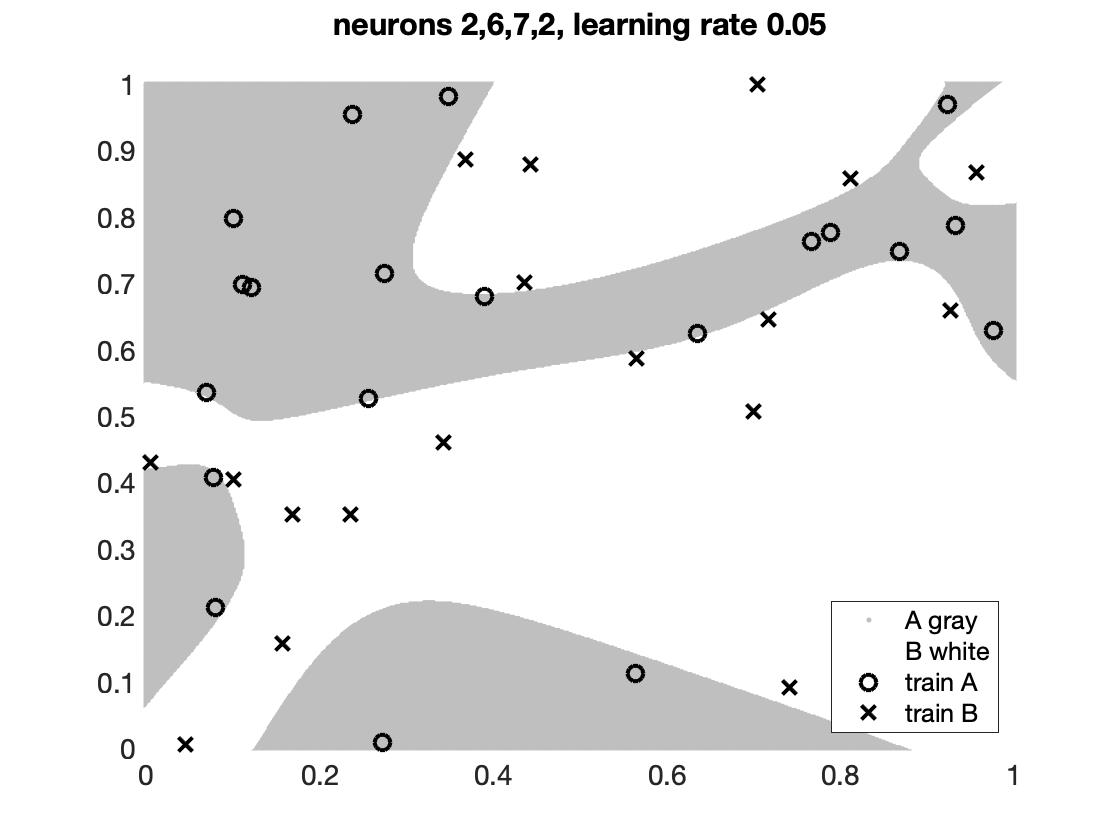
\includegraphics[width=1\textwidth]{q12.jpg}
\end{figure}	

\subsubsection*{Summarize}
\begin{itemize}
\item The more neurons the hidden layers have, the more accuracy of this output of this system.
\item When iteration number = 1e5, there is no useful output.
\item It seems the accuracy stop increasing on some thershold of some parametor.
\item The time consumed by this module highly depends on the iterations steps.
\end{itemize}

\subsection*{Problem 2}
\subsection*{(a)}
\begin{figure}[H]
  	\centering
  	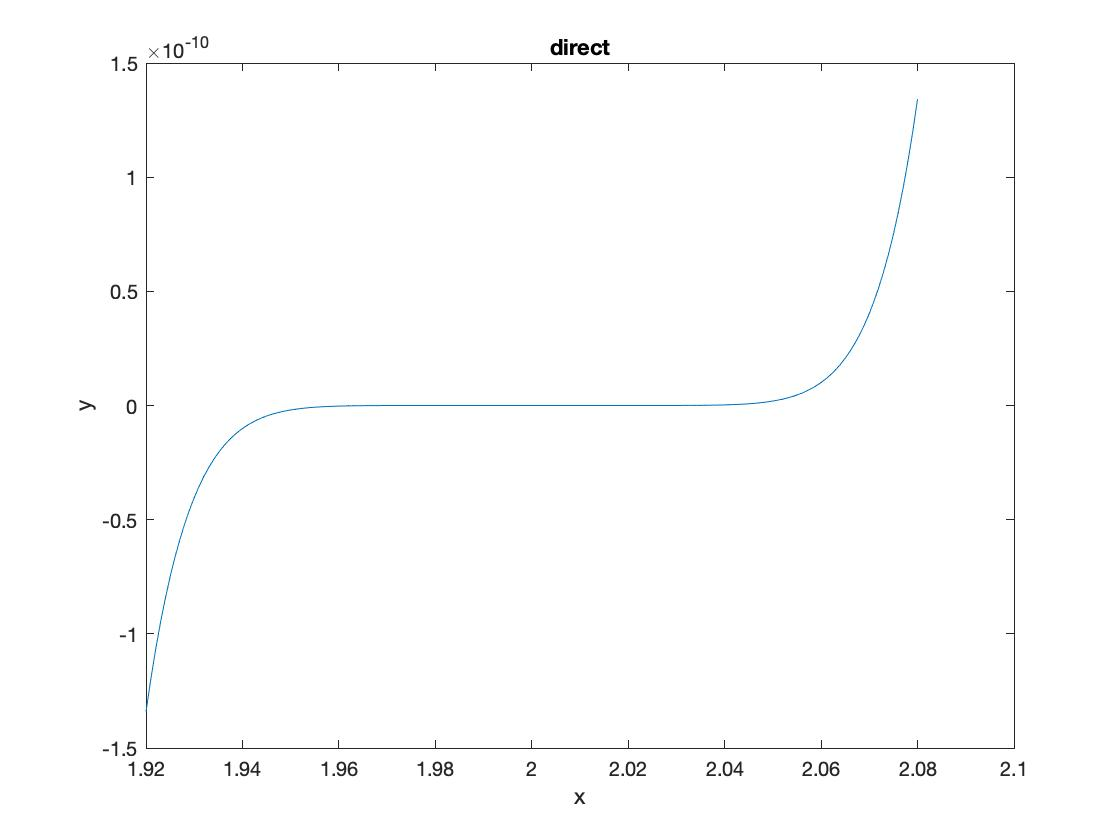
\includegraphics[width=0.6\textwidth]{q2a1.jpg}
\end{figure}	
\begin{figure}[H]
  	\centering
  	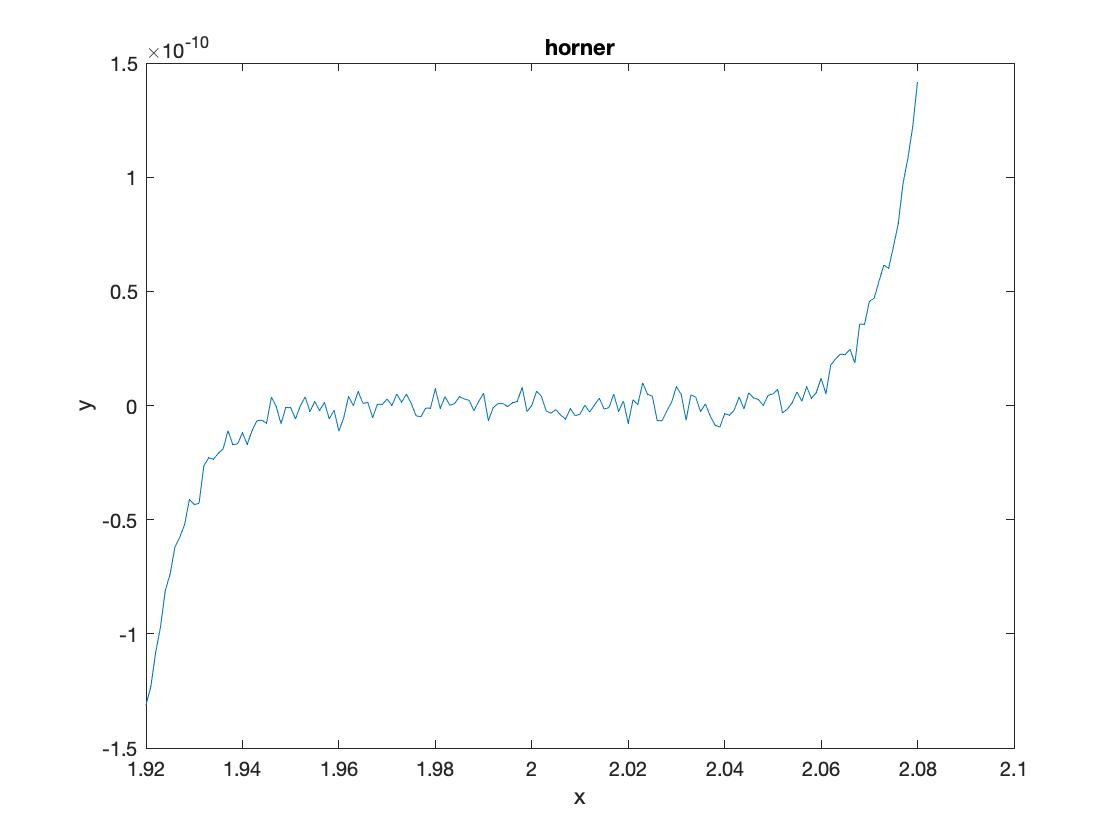
\includegraphics[width=0.6\textwidth]{q2a2.jpg}
\end{figure}	
The figure evaluated by Horner's method have more small waves, which means the evaluation using Horner's method can preserve more accuracy.

\subsection*{(b)}
\begin{lstlisting}
root = bisection(g, 1.92, 2.08, 1e-6);
fprintf("root is %6.10f\n", root);
\end{lstlisting}
output is:\\
root is 2.0000000000.
r =  1.999999.

\subsection*{(c)}
Because we loose some digits of accuracy in the intermediate steps, so the bisection function could iterate forever, then there will be no such a root.

\subsection*{(d)}
\begin{lstlisting}
r1 = fsolve(z, 1.9)
r2 = fsolve(f, 1.9)
\end{lstlisting}
output is: \\
r1 = 1.9000
r2 = 1.9000

\subsection*{Problem 3}
For system(a): Newton method: x1 = 5.000000 x2 = 4.000000\\
For system(a): Matlab solver: x1 = 11.412779 x2 = -0.896805\\
For this system, Newton's result is NOT correct, the reason is "Matrix is close to singular or badly scaled. Results may be inaccurate.  RCOND =
4.344298e-18. ".  Because the implementations uses "/" divide to solve the system, if the matrix is singular, then the matrix is too dependent, then the inverse could be bad or not existed.\\

\noindent
For system(b): Newton method: x1 = 1.666667 x2 = -0.666667
 x3 = 1.333333\\
For system(b): Matlab solver: x1 = 1.000000 x2 = 0.000000
 x3 = 2.000000\\
 For this system, Newton's result is NOT correct, the reason is "Matrix is close to singular or badly scaled. Results may be inaccurate.  RCOND =
4.344298e-18. ".  Because the implementations uses "/" divide to solve the system, if the matrix is singular, then the matrix is too dependent, then the inverse could be bad or not existed.\\
 
\noindent
For system(c): Newton method: x1 = NaN x2 = NaN x3 = NaN x4 = NaN\\
For system(c): Matlab solver: x1 = -0.002673 x2 = 0.000267 x3 = 0.000407 x4 = 0.000407\\
 For this system, Newton's method cannot provide a solution due to the matrix is singular. Because the implementations uses "/" divide to solve the system, if the matrix is singular, then the matrix is too dependent, then the inverse could be bad or not existed.\\

\noindent
For system(d): Newton method: x1 = NaN x2 = NaN\\
For system(d): Matlab solver: x1 = 0.010048 x2 = 0.010048\\
For this system, Newton's method cannot provide a solution due to the matrix is singular. Because the implementations uses "/" divide to solve the system, if the matrix is singular, then the matrix is too dependent, then the inverse could be bad or not existed.\\

\subsection*{Problem 4}
\begin{figure}[H]
  	\centering
  	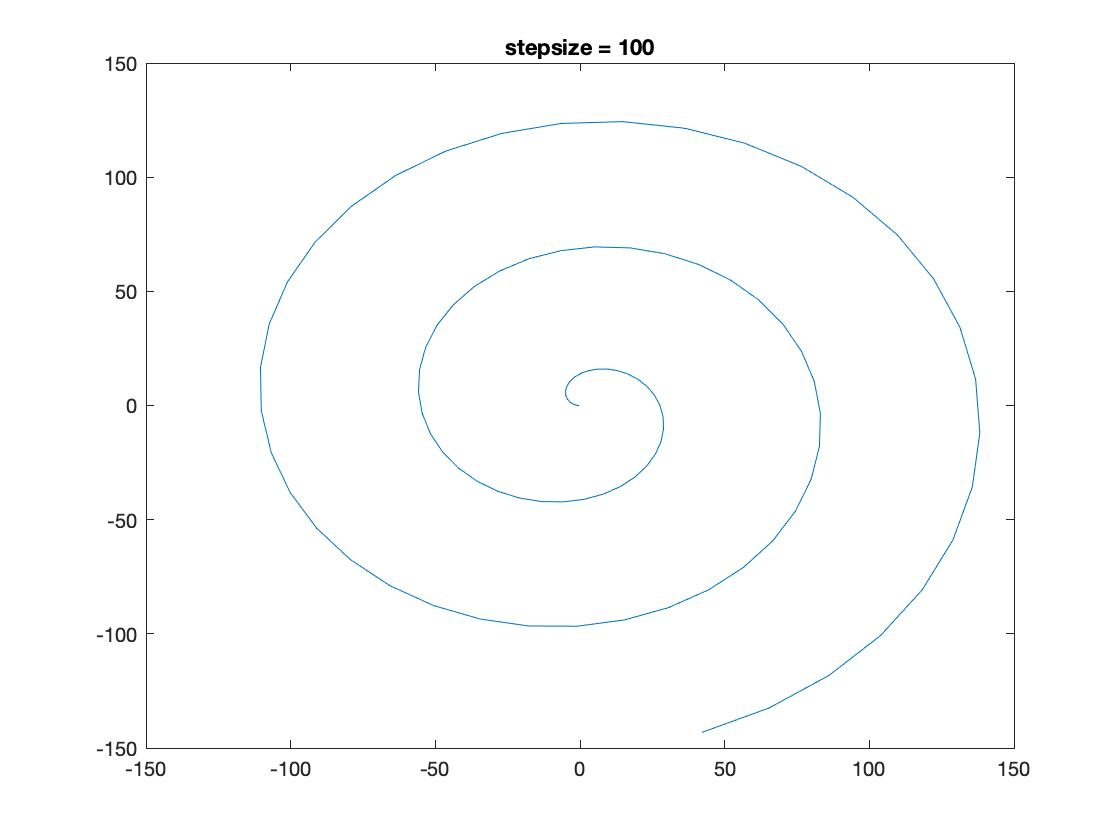
\includegraphics[width=0.6\textwidth]{q41.jpg}
\end{figure}	

\begin{figure}[H]
  	\centering
  	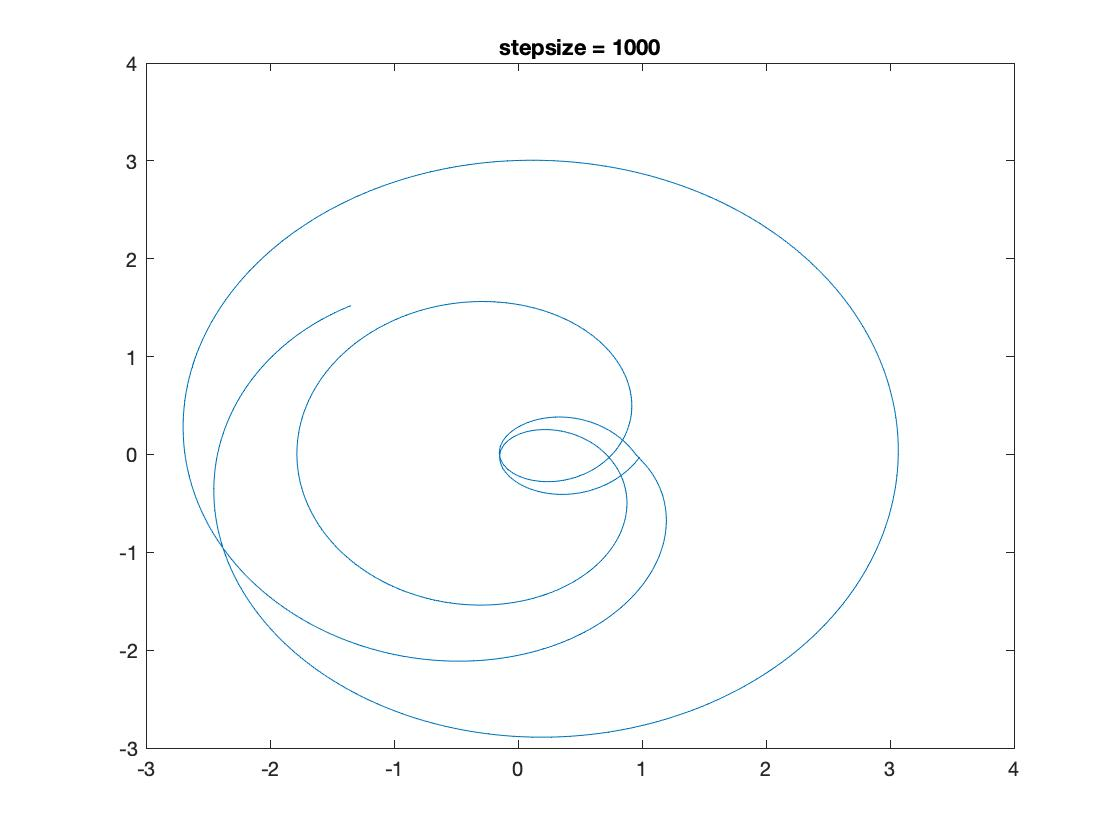
\includegraphics[width=0.6\textwidth]{q42.jpg}
\end{figure}	

\begin{figure}[H]
  	\centering
  	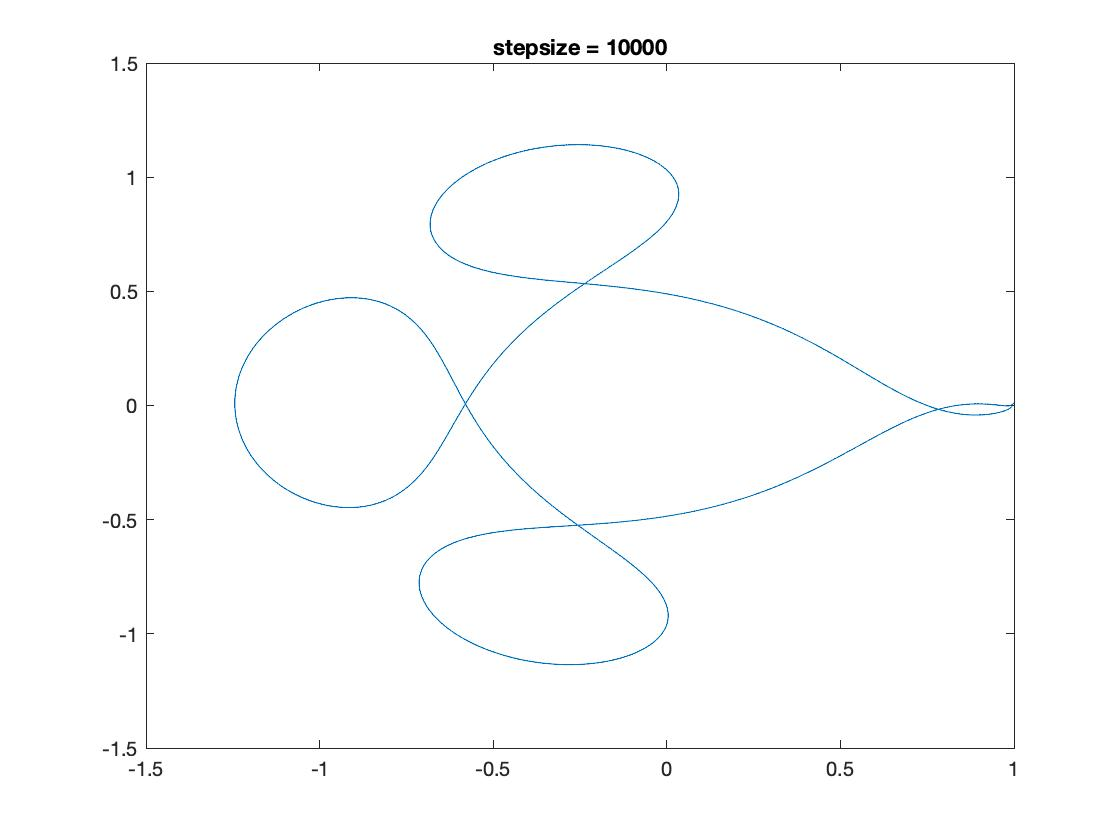
\includegraphics[width=0.6\textwidth]{q43.jpg}
\end{figure}	

\begin{figure}[H]
  	\centering
  	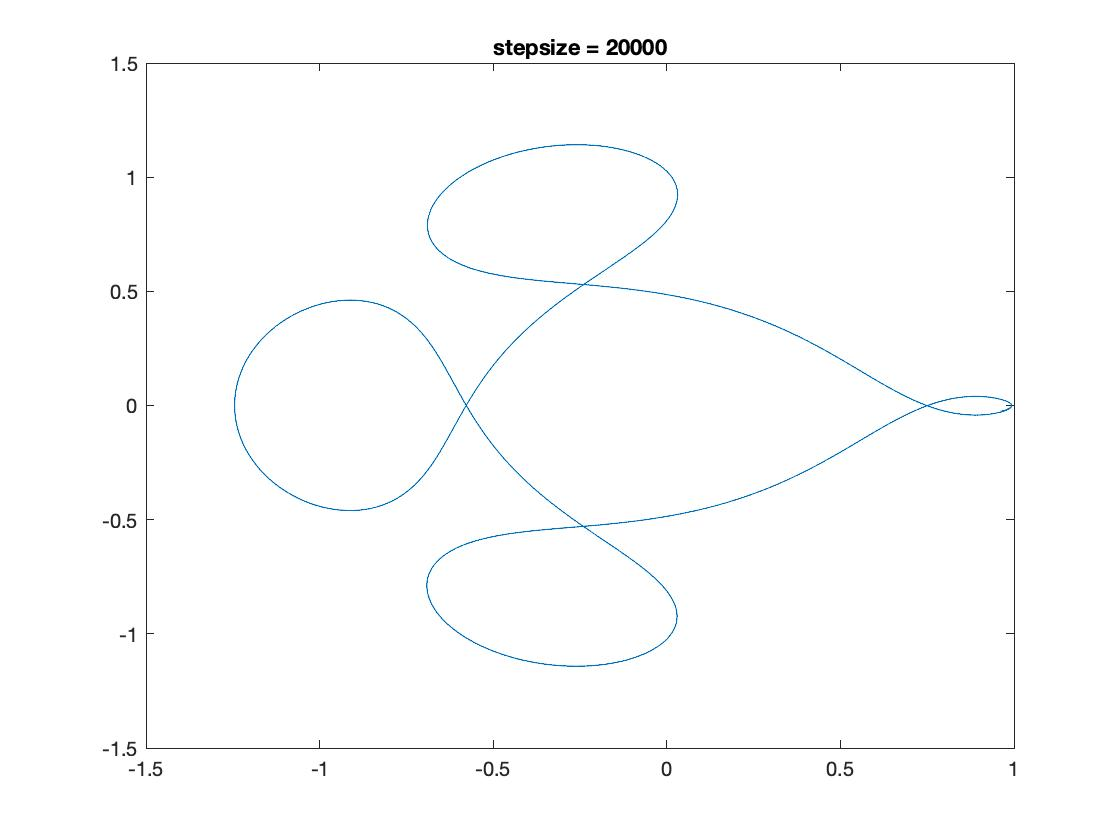
\includegraphics[width=0.6\textwidth]{q44.jpg}
\end{figure}	

How many uniform steps are needed before the orbit appears to be qualitatively correct?\\
Bases on the experiment, "stepsize = 10000" is needed before the orbit appears to be qualitatively correct.

\subsection*{Problem 5}
\begin{lstlisting}
                                        number of
                      ---------------------------------------------
solver    CPU time    steps    failed steps    function evaluations
ode23     8.8339    1.2156e+06   0.0000e+00    3.6467e+06
ode45     0.5089    3.9039e+04   4.7000e+01    2.3452e+05
ode78     0.4882    9.9650e+03   2.9300e+02    1.7292e+05
ode89     0.2598    3.6840e+03   5.5000e+01    7.8189e+04
ode113    0.3613    1.7789e+04   2.2600e+02    3.5805e+04
\end{lstlisting}

\noindent
ode89 is the most efficient solver on this problem.

\subsection*{Problem 6}
\subsubsection*{a}
\begin{figure}[H]
  	\centering
  	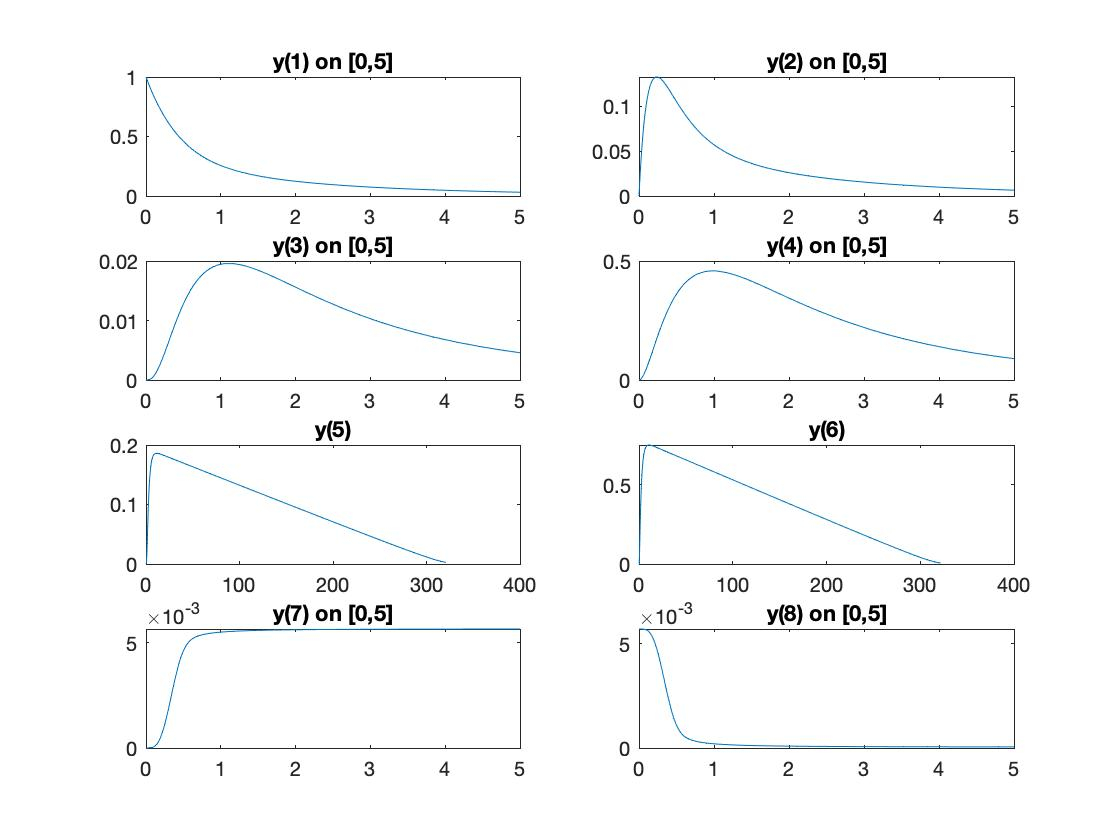
\includegraphics[width=1\textwidth]{q6a.jpg}
\end{figure}	

\subsubsection*{b}
Note: the table' width is too large, so I include the screenshot here.
\begin{figure}[H]
  	\centering
  	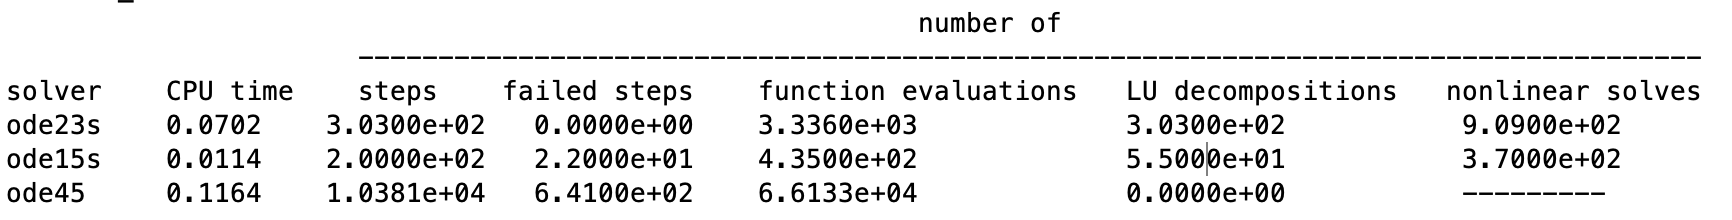
\includegraphics[width=1\textwidth]{q6b.png}
\end{figure}	

\subsubsection*{c}
For solving stiff and non-linear differential equations, the ode15s solver is the most efficient one.

\subsection*{Problem 7}
\subsubsection*{(a)}
translate the data to a time series with t is the time array and xyz is the matrix constituted of [x, y, z].\\
use matlab's time series function to interpolate this time series by a day.\\
while T < maxtime, check $(x[T] - x[0])^2 + (y[T] - y[0])^2 + (z[T] - z[0])^2 <= tolerant.$, then increment T by 10 days.\\
return the minimum T.\\

\lstinputlisting{findPeriod.m}

\subsubsection*{(b)}



\subsection*{Problem 8}
\begin{figure}[H]
  	\centering
  	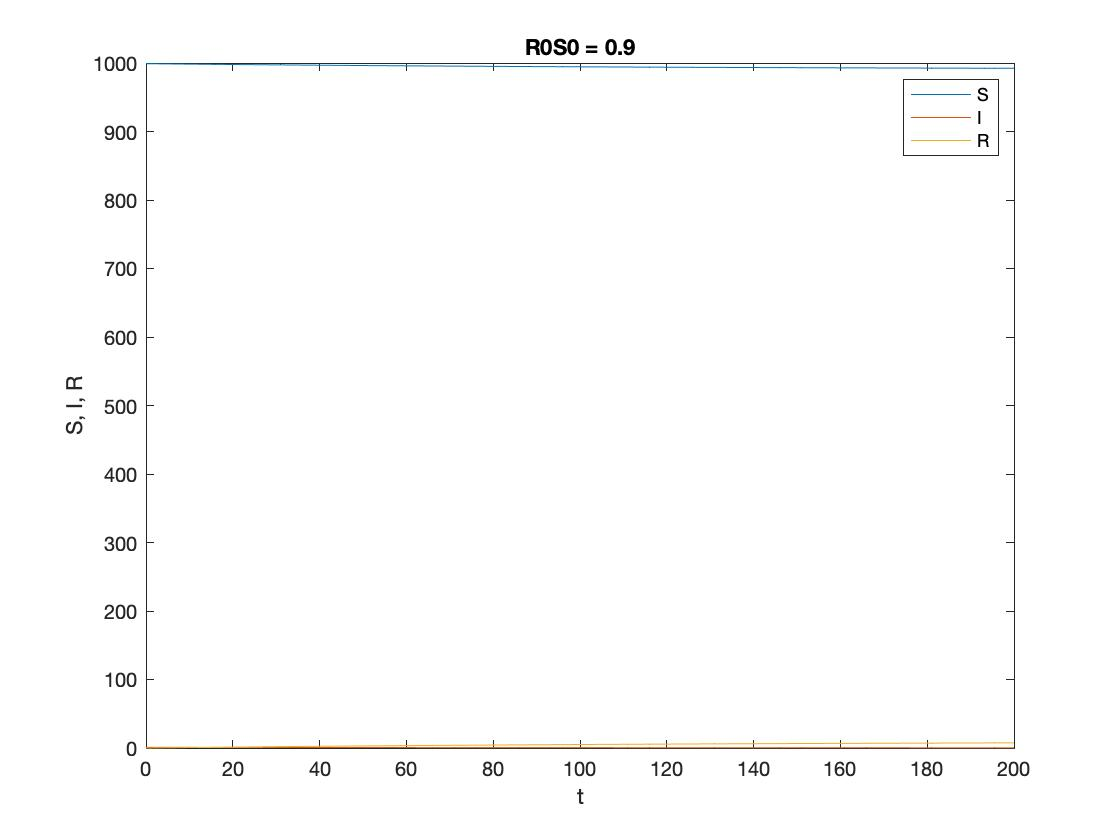
\includegraphics[width=0.8\textwidth]{q81.jpg}
\end{figure}	

\begin{figure}[H]
  	\centering
  	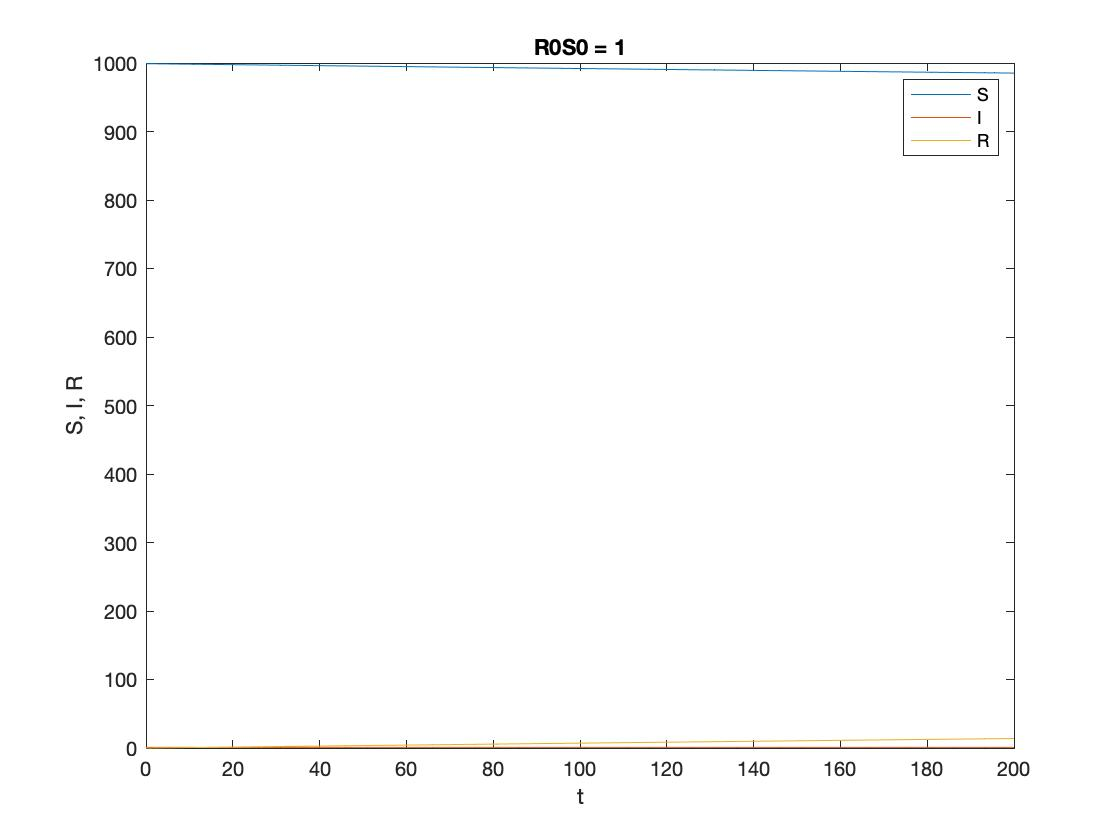
\includegraphics[width=0.8\textwidth]{q82.jpg}
\end{figure}	

\begin{figure}[H]
  	\centering
  	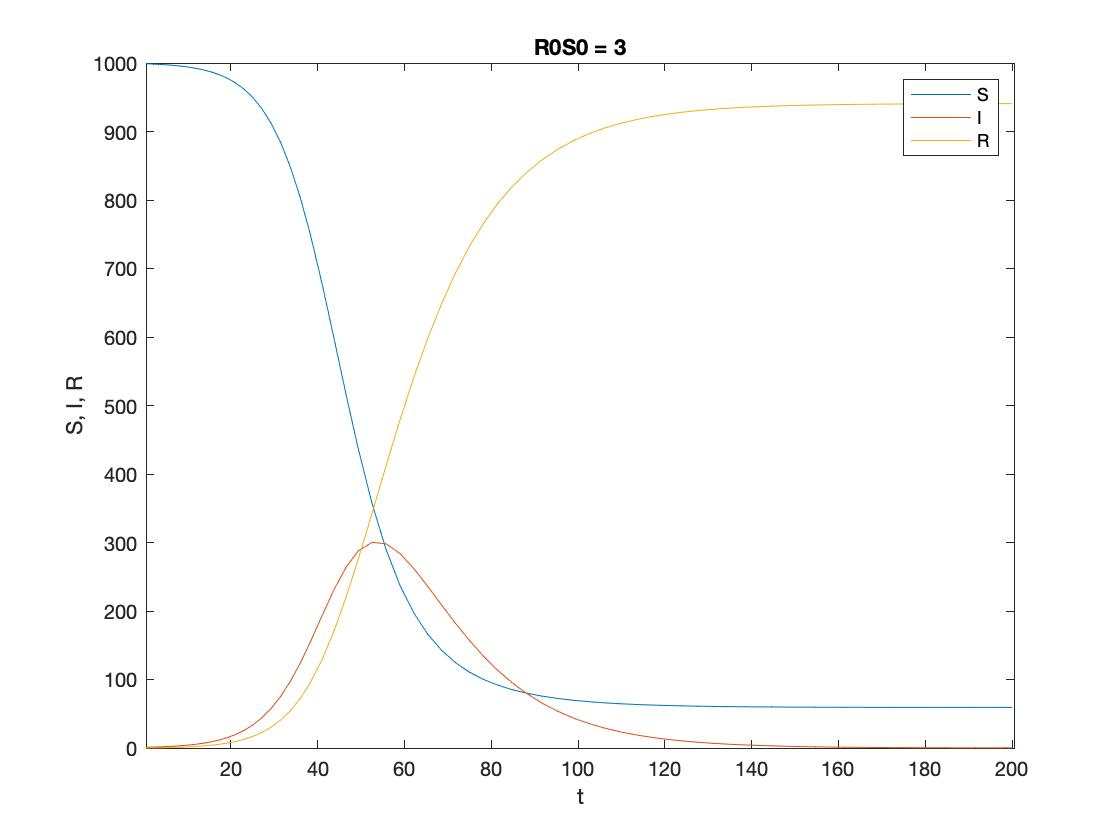
\includegraphics[width=0.8\textwidth]{q83.jpg}
\end{figure}	

\begin{figure}[H]
  	\centering
  	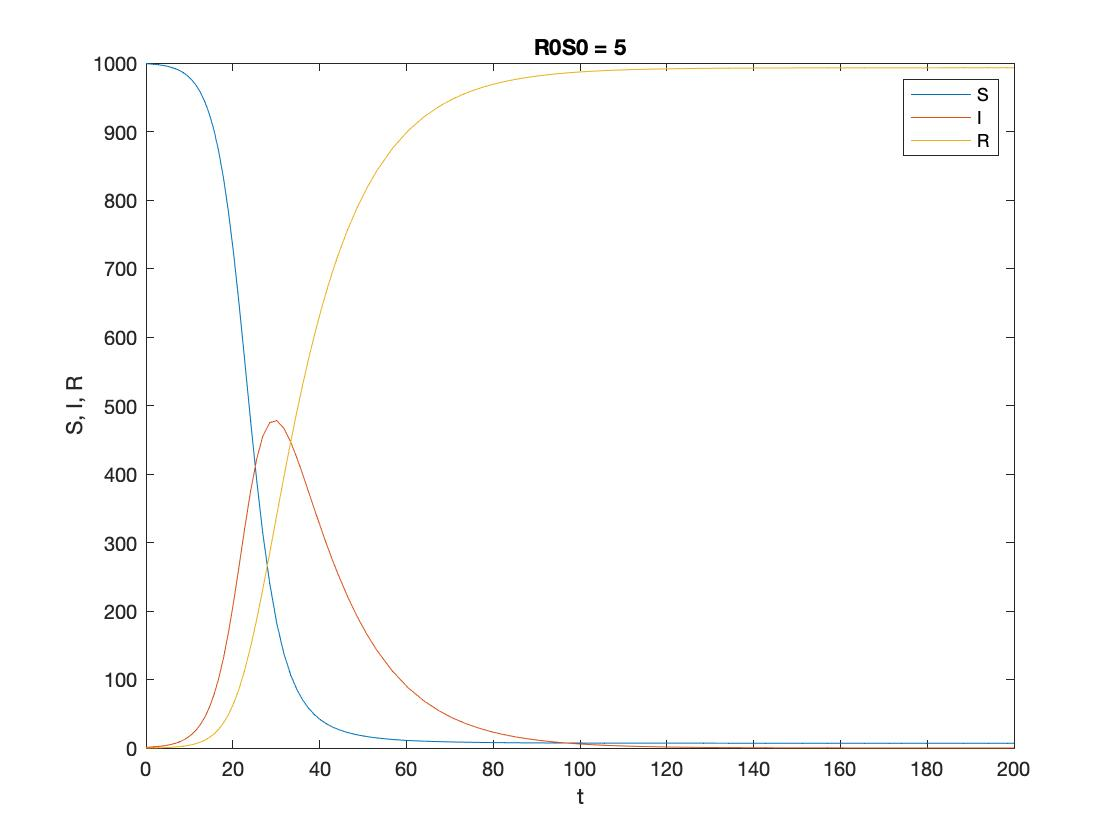
\includegraphics[width=0.8\textwidth]{q84.jpg}
\end{figure}	


\end{document}


